\documentclass[]{book}
\usepackage{lmodern}
\usepackage{amssymb,amsmath}
\usepackage{ifxetex,ifluatex}
\usepackage{fixltx2e} % provides \textsubscript
\ifnum 0\ifxetex 1\fi\ifluatex 1\fi=0 % if pdftex
  \usepackage[T1]{fontenc}
  \usepackage[utf8]{inputenc}
\else % if luatex or xelatex
  \ifxetex
    \usepackage{mathspec}
  \else
    \usepackage{fontspec}
  \fi
  \defaultfontfeatures{Ligatures=TeX,Scale=MatchLowercase}
\fi
% use upquote if available, for straight quotes in verbatim environments
\IfFileExists{upquote.sty}{\usepackage{upquote}}{}
% use microtype if available
\IfFileExists{microtype.sty}{%
\usepackage{microtype}
\UseMicrotypeSet[protrusion]{basicmath} % disable protrusion for tt fonts
}{}
\usepackage[margin=1in]{geometry}
\usepackage{hyperref}
\hypersetup{unicode=true,
            pdftitle={CNC Fly Food Dispenser},
            pdfauthor={Matt Wayland},
            pdfborder={0 0 0},
            breaklinks=true}
\urlstyle{same}  % don't use monospace font for urls
\usepackage{natbib}
\bibliographystyle{apalike}
\usepackage{longtable,booktabs}
\usepackage{graphicx,grffile}
\makeatletter
\def\maxwidth{\ifdim\Gin@nat@width>\linewidth\linewidth\else\Gin@nat@width\fi}
\def\maxheight{\ifdim\Gin@nat@height>\textheight\textheight\else\Gin@nat@height\fi}
\makeatother
% Scale images if necessary, so that they will not overflow the page
% margins by default, and it is still possible to overwrite the defaults
% using explicit options in \includegraphics[width, height, ...]{}
\setkeys{Gin}{width=\maxwidth,height=\maxheight,keepaspectratio}
\IfFileExists{parskip.sty}{%
\usepackage{parskip}
}{% else
\setlength{\parindent}{0pt}
\setlength{\parskip}{6pt plus 2pt minus 1pt}
}
\setlength{\emergencystretch}{3em}  % prevent overfull lines
\providecommand{\tightlist}{%
  \setlength{\itemsep}{0pt}\setlength{\parskip}{0pt}}
\setcounter{secnumdepth}{5}
% Redefines (sub)paragraphs to behave more like sections
\ifx\paragraph\undefined\else
\let\oldparagraph\paragraph
\renewcommand{\paragraph}[1]{\oldparagraph{#1}\mbox{}}
\fi
\ifx\subparagraph\undefined\else
\let\oldsubparagraph\subparagraph
\renewcommand{\subparagraph}[1]{\oldsubparagraph{#1}\mbox{}}
\fi

%%% Use protect on footnotes to avoid problems with footnotes in titles
\let\rmarkdownfootnote\footnote%
\def\footnote{\protect\rmarkdownfootnote}

%%% Change title format to be more compact
\usepackage{titling}

% Create subtitle command for use in maketitle
\newcommand{\subtitle}[1]{
  \posttitle{
    \begin{center}\large#1\end{center}
    }
}

\setlength{\droptitle}{-2em}
  \title{CNC Fly Food Dispenser}
  \pretitle{\vspace{\droptitle}\centering\huge}
  \posttitle{\par}
  \author{Matt Wayland}
  \preauthor{\centering\large\emph}
  \postauthor{\par}
  \predate{\centering\large\emph}
  \postdate{\par}
  \date{2017-07-03}

\usepackage{booktabs}
\usepackage{amsthm}
\makeatletter
\def\thm@space@setup{%
  \thm@preskip=8pt plus 2pt minus 4pt
  \thm@postskip=\thm@preskip
}
\makeatother

\usepackage{amsthm}
\newtheorem{theorem}{Theorem}[chapter]
\newtheorem{lemma}{Lemma}[chapter]
\theoremstyle{definition}
\newtheorem{definition}{Definition}[chapter]
\newtheorem{corollary}{Corollary}[chapter]
\newtheorem{proposition}{Proposition}[chapter]
\theoremstyle{definition}
\newtheorem{example}{Example}[chapter]
\theoremstyle{remark}
\newtheorem*{remark}{Remark}
\begin{document}
\maketitle

{
\setcounter{tocdepth}{1}
\tableofcontents
}
\chapter*{Preface}\label{preface}
\addcontentsline{toc}{chapter}{Preface}

\begin{center}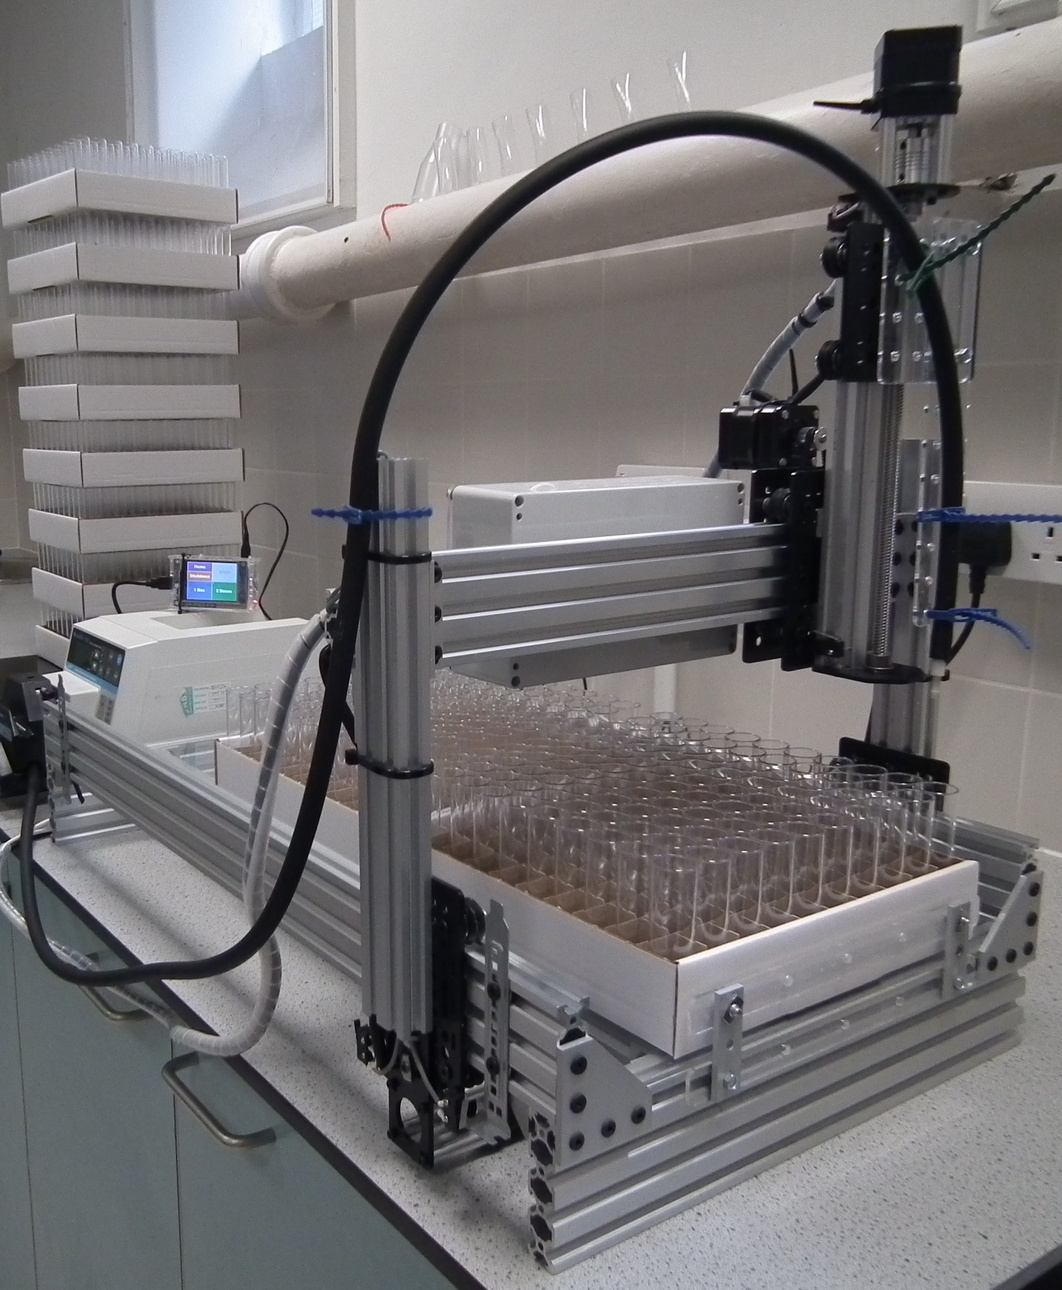
\includegraphics[width=0.75\linewidth]{images/system} \end{center}

\section*{Github}\label{github}
\addcontentsline{toc}{section}{Github}

\href{https://github.com/WaylandM/fly-food-robot}{WaylandM/fly-food-robot}

\section*{License}\label{license}
\addcontentsline{toc}{section}{License}

License for software and documentation:
\href{https://www.gnu.org/licenses/gpl-3.0.en.html}{GPL-3}

\section*{Contact}\label{contact}
\addcontentsline{toc}{section}{Contact}

Matt Wayland

\section*{Colophon}\label{colophon}
\addcontentsline{toc}{section}{Colophon}

This book was produced using the \textbf{bookdown} package
\citep{R-bookdown}, which was built on top of R Markdown and
\textbf{knitr} \citep{xie2015}.

\chapter{Introduction}\label{intro}

The fruit fly, \emph{Drosophila melanogaster}, is one of the most
important model organisms in biological research. Maintaining stocks of
fruit flies in the laboratory is labour-intensive. One task which lends
itself to automation is the production of the vials of food in which the
flies are reared. Fly facilities typically have to generate several
thousand vials of fly food each week to sustain their fly stocks. The
system presented here combines a cartesian coordinate robot with a
peristaltic pump. The design of the robot is based on the Routy CNC
Router created by Mark Carew
(\url{http://openbuilds.org/builds/routy-cnc-router-v-slot-belt-pinion.101/}),
and uses belt and pully actuators for the X and Y axes, and a leadscrew
actuator for the Z axis. CNC motion and operation of the peristaltic
pump are controlled by grbl (\url{https://github.com/gnea/grbl}), an
open source, embedded, high performance g-code parser. Grbl is written
in optimized C and runs directly on an Arduino. A Raspberry Pi is used
to generate and stream G-code instructions to Grbl. A touch screen on
the Raspberry Pi provides a graphical user interface to the system. This
manual explains how to install the required software and operate the
robot. Instructions for building the hardware are available on
\href{http://docubricks.com/viewer.jsp?id=8652757760093769728}{DocuBricks}.

A Raspberry Pi is used to generate and stream G-code to the Arduino. A
touch screen on the Raspberry Pi provides the user interface; a
resistive rather than capacitive touch screen was chosen so that it
could be operated by a person wearing gloves.

\chapter{Grbl installation and
configuration}\label{grbl-installation-and-configuration}

\section{Overview}\label{overview}

CNC motion control is provided by grbl
(\url{https://github.com/gnea/grbl}), an open source, embedded, high
performance g-code parser. Grbl is written in optimized C and runs
directly on an Arduino. This is used in conjunction with the gShield
(formerly known as grblshield) which provides the hardware drivers for
the stepper motors. Grbl sends out TTL signals on pins A3 and 13 or the
Arduino to control coolant flow and spindle direction, respectively.
Here these signals are used to remotely control a peristaltic pump.

\section{Flashing Grbl to Arduino}\label{flashing-grbl-to-arduino}

To flash Grbl to the Arduino you will need a computer with the latest
version of the \href{https://www.arduino.cc/en/Main/Software}{Arduino
IDE} installed. The following instructions for flashing Grbl to the
Arduino are taken from:
\url{https://github.com/gnea/grbl/wiki/Compiling-Grbl}

\emph{\textbf{NOTE: Before starting, delete prior Grbl library
installations from the Arduino IDE. Otherwise, you'll have compiling
issues! On a Mac, Arduino libraries are located in
\texttt{\textasciitilde{}/Documents/Arduino/libraries/}. On Windows,
it's in
\texttt{My\ Documents\textbackslash{}Arduino\textbackslash{}libraries}.}}

\begin{enumerate}
\def\labelenumi{\arabic{enumi}.}
\tightlist
\item
  Download the Grbl source code.
\end{enumerate}

\begin{itemize}
\tightlist
\item
  Open the following page in your web browser:
  \url{https://github.com/gnea/grbl}
\item
  Click on the \texttt{\textless{}\textgreater{}Code} Tab
\item
  Click the \texttt{Clone\ or\ Download} green button on the Grbl home
  page.
\item
  Click the \texttt{Download\ ZIP}
\item
  Unzip the download and you'll have a folder called \texttt{grbl-XXX},
  where \texttt{XXX} is the release version.
\end{itemize}

\begin{enumerate}
\def\labelenumi{\arabic{enumi}.}
\setcounter{enumi}{1}
\tightlist
\item
  Launch the Arduino IDE
\end{enumerate}

\begin{itemize}
\tightlist
\item
  Make sure you are using the most recent version of the Arduino IDE!
\end{itemize}

\begin{figure}

{\centering 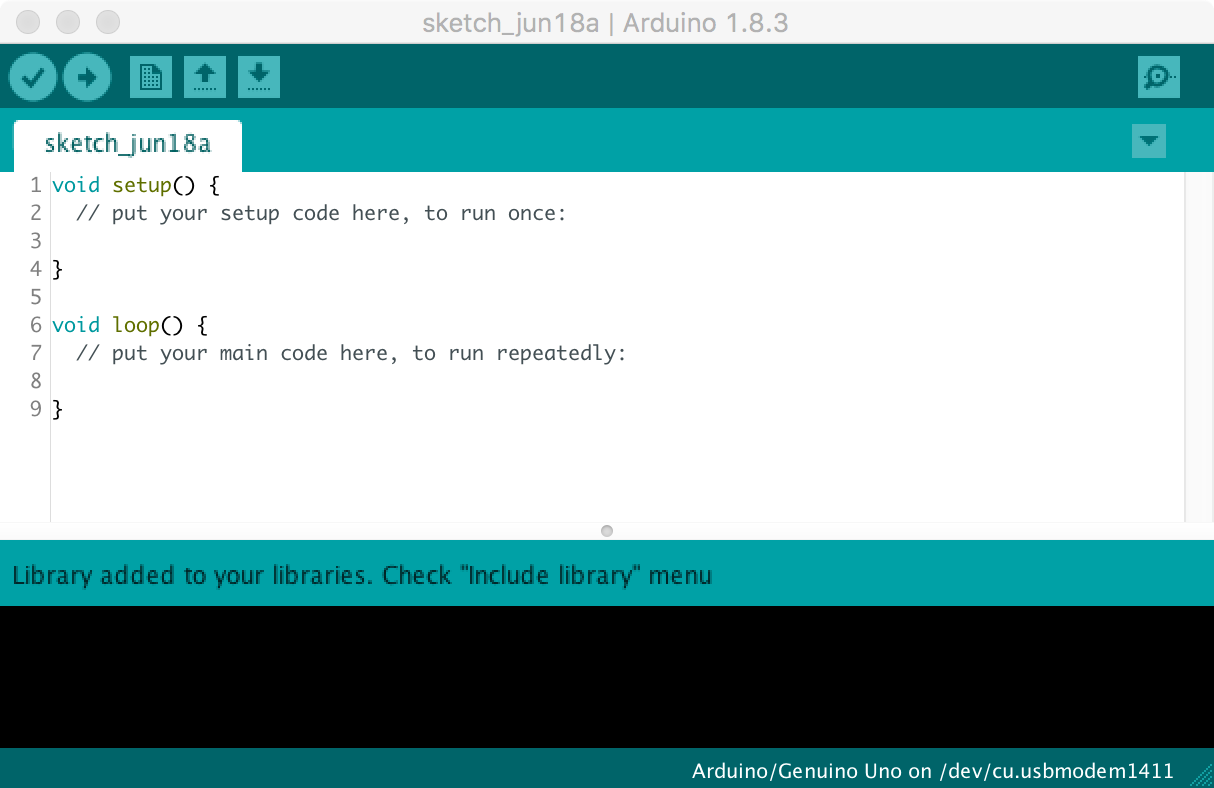
\includegraphics[width=0.75\linewidth]{images/arduino_IDE} 

}

\caption{Arduino IDE}\label{fig:arduinoIDE}
\end{figure}

\begin{enumerate}
\def\labelenumi{\arabic{enumi}.}
\setcounter{enumi}{2}
\tightlist
\item
  Load Grbl into the Arduino IDE as a Library.
\end{enumerate}

\begin{itemize}
\tightlist
\item
  Click the \texttt{Sketch} drop-down menu, navigate to
  \texttt{Include\ Library} and select \texttt{Add\ .ZIP\ Library}.
\item
  \textbf{IMPORTANT:} Select the \texttt{Grbl} folder
  \textbf{\emph{inside}} the \texttt{grbl-XXX} folder, which
  \textbf{only} contains the source files and an example directory.
\end{itemize}

\begin{figure}

{\centering 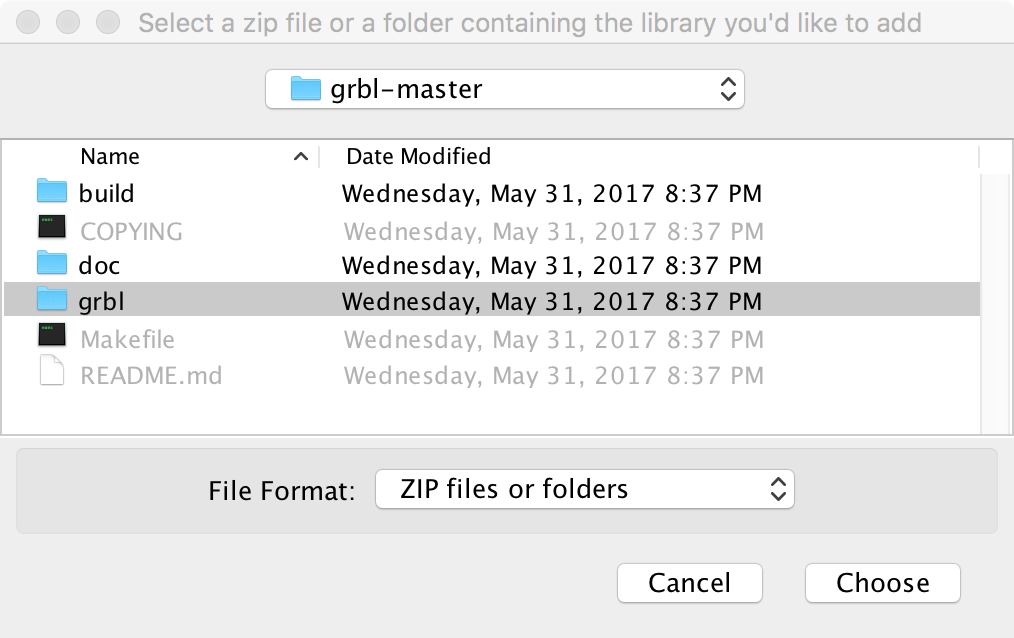
\includegraphics[width=0.75\linewidth]{images/add_grbl_lib} 

}

\caption{Loading Grbl library into the Arduino IDE}\label{fig:addGrblLib}
\end{figure}

\begin{itemize}
\tightlist
\item
  If you accidentally select the \texttt{.zip} file or the wrong folder,
  you will need to navigate to your Arduino library, delete the mistake,
  and re-do Step 3.
\end{itemize}

\begin{enumerate}
\def\labelenumi{\arabic{enumi}.}
\setcounter{enumi}{3}
\tightlist
\item
  Open the \texttt{GrblUpload} Arduino example.
\end{enumerate}

\begin{itemize}
\tightlist
\item
  Click the \texttt{File} drop-down menu, navigate to
  \texttt{Examples-\textgreater{}Grbl}, and select \texttt{GrblUpload}.
\end{itemize}

\begin{figure}

{\centering 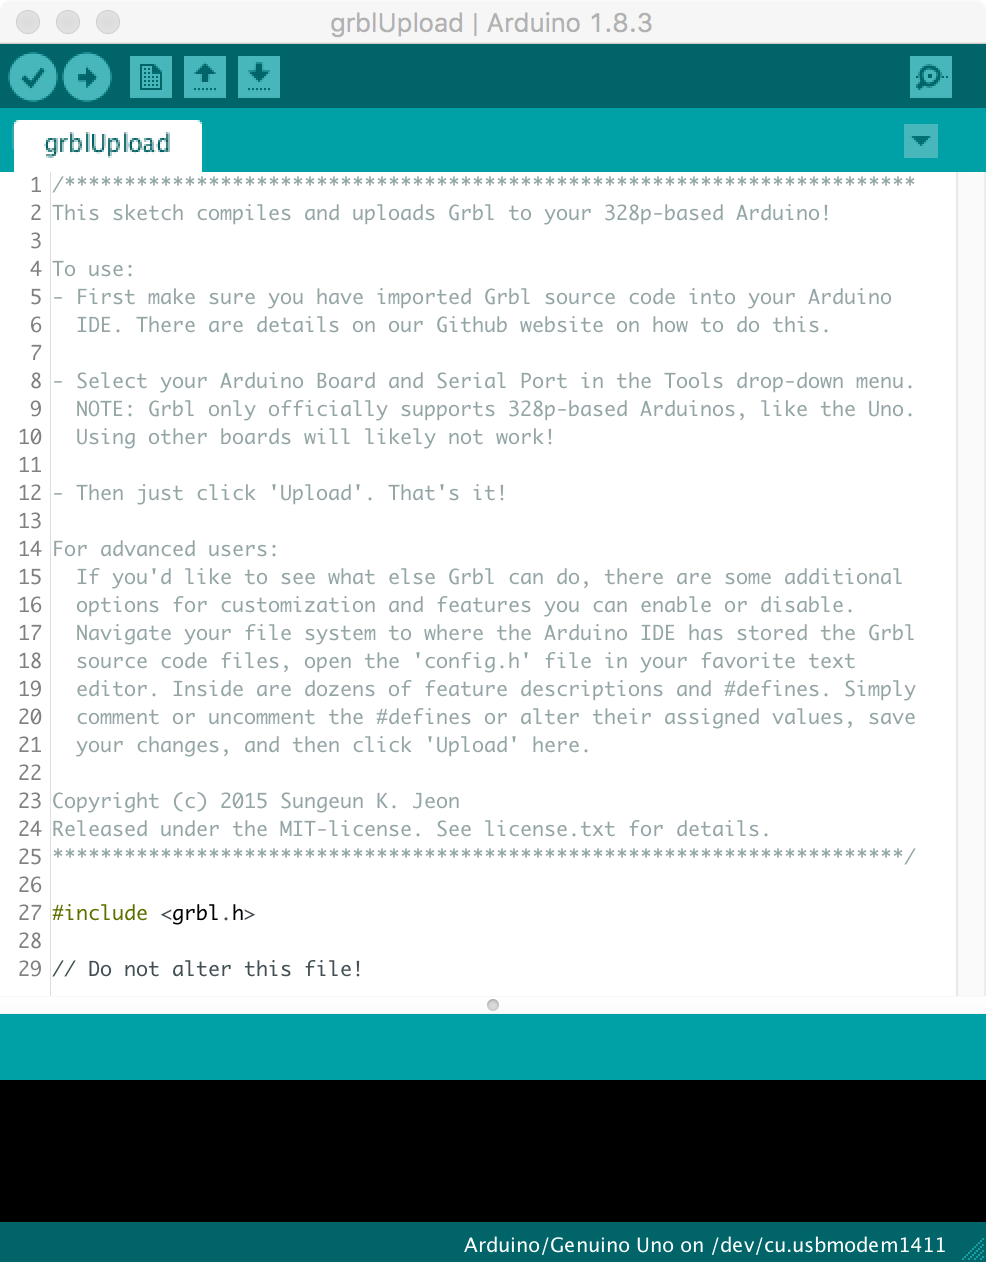
\includegraphics[width=0.75\linewidth]{images/grbl_upload_file} 

}

\caption{GrblUpload example file}\label{fig:grblUploadFile}
\end{figure}

\begin{enumerate}
\def\labelenumi{\arabic{enumi}.}
\setcounter{enumi}{4}
\tightlist
\item
  Compile and upload Grbl to your Arduino.
\end{enumerate}

\begin{itemize}
\tightlist
\item
  Connect your computer directly to the Arduino using the USB cable.
\end{itemize}

\begin{figure}

{\centering 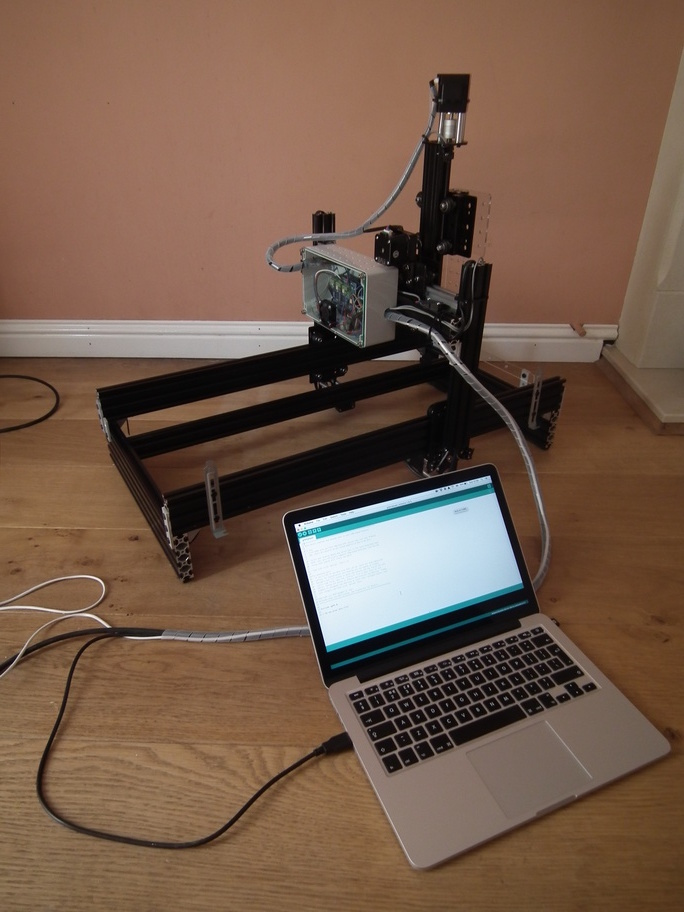
\includegraphics[width=0.75\linewidth]{images/laptop_connected_to_arduino} 

}

\caption{Laptop connected directly to Arduino}\label{fig:laptop2arduino}
\end{figure}

\begin{itemize}
\tightlist
\item
  Make sure your board is set to the Arduino Uno in the
  \texttt{Tool-\textgreater{}Board} menu and the serial port is selected
  correctly in \texttt{Tool-\textgreater{}Serial\ Port}.
\item
  Click the \texttt{Upload}, and Grbl should compile and flash to your
  Arduino! (Flashing with a programmer also works by using the
  \texttt{Upload\ Using\ Programmer} menu command.)
\end{itemize}

\section{Check serial connection to
Grbl}\label{check-serial-connection-to-grbl}

\emph{\textbf{NOTE: Before powering up the gShield and motors, check
that the actuator carriages for all three axes are approximately
centred. Initially we do not know in which direction the actuator
carriages will travel when G-code commands are issued, so positioning
each in the middle of its range reduces the risk of collisions with the
end stops.}}

\begin{figure}

{\centering 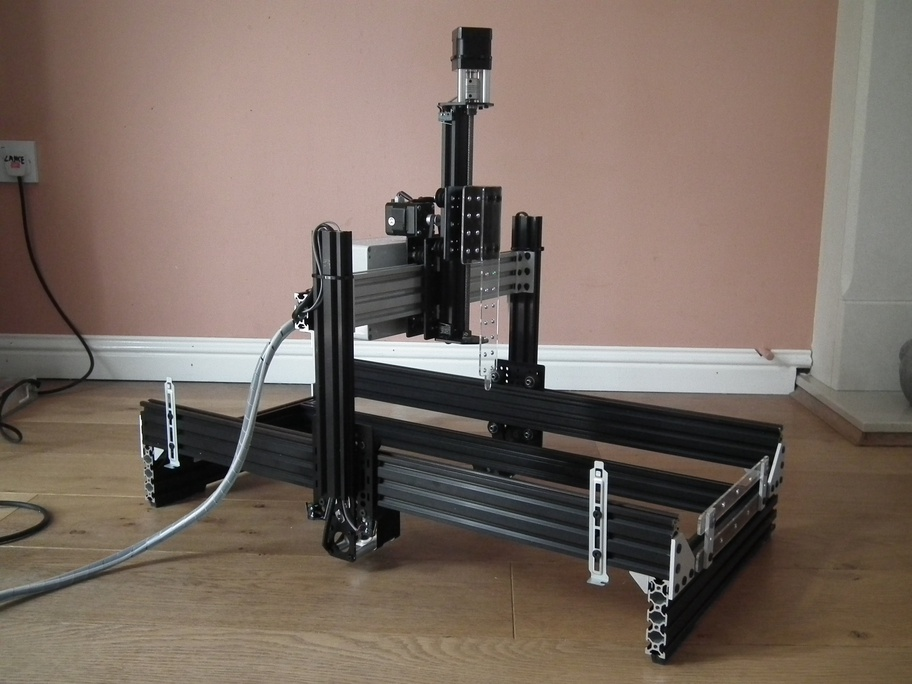
\includegraphics[width=0.75\linewidth]{images/actuator_carriages_centred} 

}

\caption{Actuator carriages centred in preparation for powering-up motors for first time}\label{fig:actuatorsCentred}
\end{figure}

\begin{enumerate}
\def\labelenumi{\arabic{enumi}.}
\tightlist
\item
  Open serial monitor in Arduino IDE
\end{enumerate}

\begin{itemize}
\tightlist
\item
  Click \texttt{Tools} drop-down menu, and select
  \texttt{Serial\ Monitor}
\end{itemize}

\begin{figure}

{\centering \includegraphics[width=0.75\linewidth]{images/Arduino_IDE_serial_monitor} 

}

\caption{Arduino IDE Serial Monitor}\label{fig:serialMonitor}
\end{figure}

\begin{itemize}
\tightlist
\item
  Note that line-ending is set to \texttt{Carriage\ return} and baud
  rate is set to \texttt{115200}
\end{itemize}

\begin{enumerate}
\def\labelenumi{\arabic{enumi}.}
\setcounter{enumi}{1}
\tightlist
\item
  Try issuing a G-code command.
\end{enumerate}

\begin{itemize}
\tightlist
\item
  Type \texttt{?} and hit return.
\item
  This command will report the current position; as we have just started
  the system up all axes will be at 0.000.
\end{itemize}

\begin{enumerate}
\def\labelenumi{\arabic{enumi}.}
\setcounter{enumi}{2}
\tightlist
\item
  Now try moving actuators
\end{enumerate}

\begin{itemize}
\tightlist
\item
  To move in the x-axis type \texttt{x5} and hit return. Make a note of
  the direction in which the actuator carriage moves. N.B. this command
  tells Grbl to move to the x coordinate that is 5 units from the
  origin, it is not equivalent to telling the robot to move 5 units in
  the x-axis.
\item
  To move in the opposite direction along the x-axis type \texttt{x-5}
  and hit return.
\item
  To return to the starting point, use \texttt{x0}
\item
  Repeat for the other axes, replacing the x in the commands with y or
  z. Make a note of the direction the actuator carriages move with each
  command.
\end{itemize}

\section{Grbl configuration}\label{grbl-configuration}

\subsection{Read current
configuration}\label{read-current-configuration}

\begin{itemize}
\tightlist
\item
  The \texttt{\$\$} command will report Grbl's current configuration.
\item
  Descriptions of these settings can be found here:
  \url{https://github.com/gnea/grbl/wiki/Grbl-v1.1-Configuration}
\item
  These settings will be modified in subsequent steps.
\end{itemize}

\subsection{Check directionality of each
axis.}\label{check-directionality-of-each-axis.}

\begin{figure}

{\centering 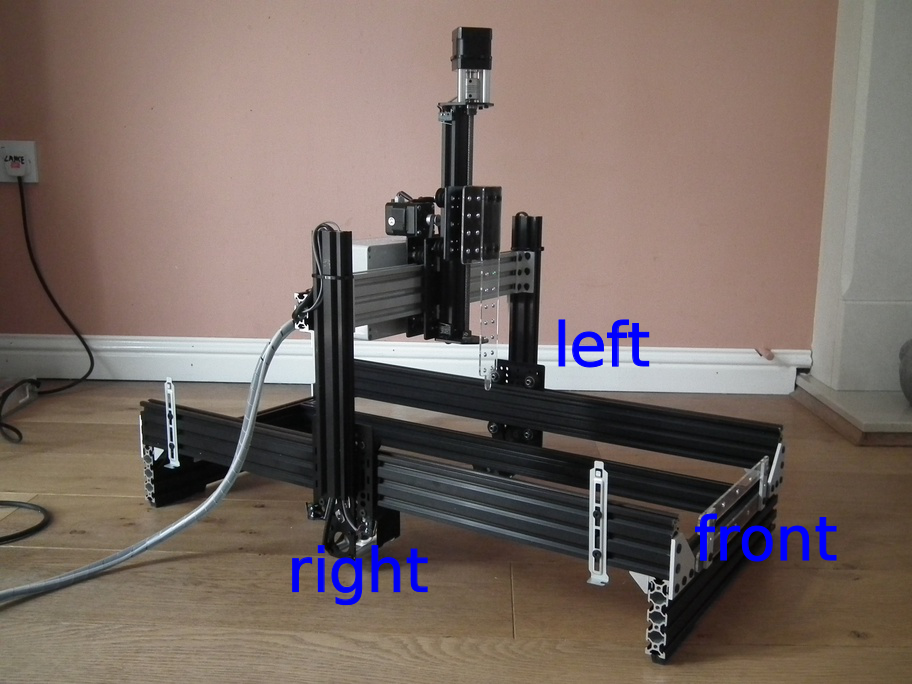
\includegraphics[width=0.75\linewidth]{images/robot_orientation} 

}

\caption{Orientation of robot.}\label{fig:robotOrientation}
\end{figure}

\begin{itemize}
\tightlist
\item
  At present the origins of all three axes are mid-way along each
  actuator, because this was the position of the actuator carriages when
  the system was started.
\item
  Make sure actuator carriages are at their current origin by entering
  this command: \texttt{x0y0z0}
\item
  Enter the command: \texttt{x5}. The x-axis carriage should move from
  right to left (orientation of robot is shown in figure
  \ref{fig:robotOrientation}. If it doesn't, make a note that it will
  need to be inverted.
\item
  Enter the command: \texttt{y5}. The y-axis carriage should move
  forwards. If it doesn't, make a note that it will need to be inverted.
\item
  Enter the command: \texttt{z5}. The z-axis carriage should move up. If
  it doesn't, make a note that it will need to be inverted.
\item
  The direction of the actuators can be inverted using setting
  \textbf{\$3}, the
  \href{https://github.com/gnea/grbl/wiki/Grbl-v1.1-Configuration\#3--direction-port-invert-mask}{Direction
  port invert (mask)}. An appropriate value is selected from table
  \ref{tab:invertMaskSettings}. For example, to invert the direction of
  the X and Z axis actuators use the following command: \texttt{\$3=5}
\end{itemize}

\begin{longtable}[]{@{}ccccc@{}}
\caption{\label{tab:invertMaskSettings} Masks for direction port
inversion.}\tabularnewline
\toprule
Setting Value & Mask & Invert X & Invert Y & Invert Z\tabularnewline
\midrule
\endfirsthead
\toprule
Setting Value & Mask & Invert X & Invert Y & Invert Z\tabularnewline
\midrule
\endhead
0 & 00000000 & N & N & N\tabularnewline
1 & 00000001 & Y & N & N\tabularnewline
2 & 00000010 & N & Y & N\tabularnewline
3 & 00000011 & Y & Y & N\tabularnewline
4 & 00000100 & N & N & Y\tabularnewline
5 & 00000101 & Y & N & Y\tabularnewline
6 & 00000110 & N & Y & Y\tabularnewline
7 & 00000111 & Y & Y & Y\tabularnewline
\bottomrule
\end{longtable}

\subsection{Activate hard limits}\label{activate-hard-limits}

Hard limits are a safety feature to prevent the machine from travelling
beyond the limits of travel. Grbl monitors the paired limit switches on
each axis and if a switch is triggered it will immediately switch off
all motors. Hard limits are activated by setting \textbf{\$21}
\href{https://github.com/gnea/grbl/wiki/Grbl-v1.1-Configuration\#21---hard-limits-boolean}{hard
limits ( boolean)} to 1:

\begin{verbatim}
$21=1
\end{verbatim}

\subsection{Setup homing}\label{setup-homing}

The homing cycle is used to set the origin of the cartesian coordinate
system used by the robot. During the homing cycle Grbl moves each
actuator in the positive direction until the limit switches are
triggered. The homing cycle is activated by setting \textbf{\$22}
\href{https://github.com/gnea/grbl/wiki/Grbl-v1.1-Configuration\#22---homing-cycle-boolean}{homing
cycle (boolean)} to 1:

\begin{verbatim}
$22=1
\end{verbatim}

Initiate a homing cycle using the following command: \texttt{\$h}. All
actuator carriages should move to the origin of their axes. The origin
of the cartesian coordinate system (home) for the robot is shown in
figures \ref{fig:xyOrigin} and \ref{fig:zOrigin}

\begin{figure}

{\centering 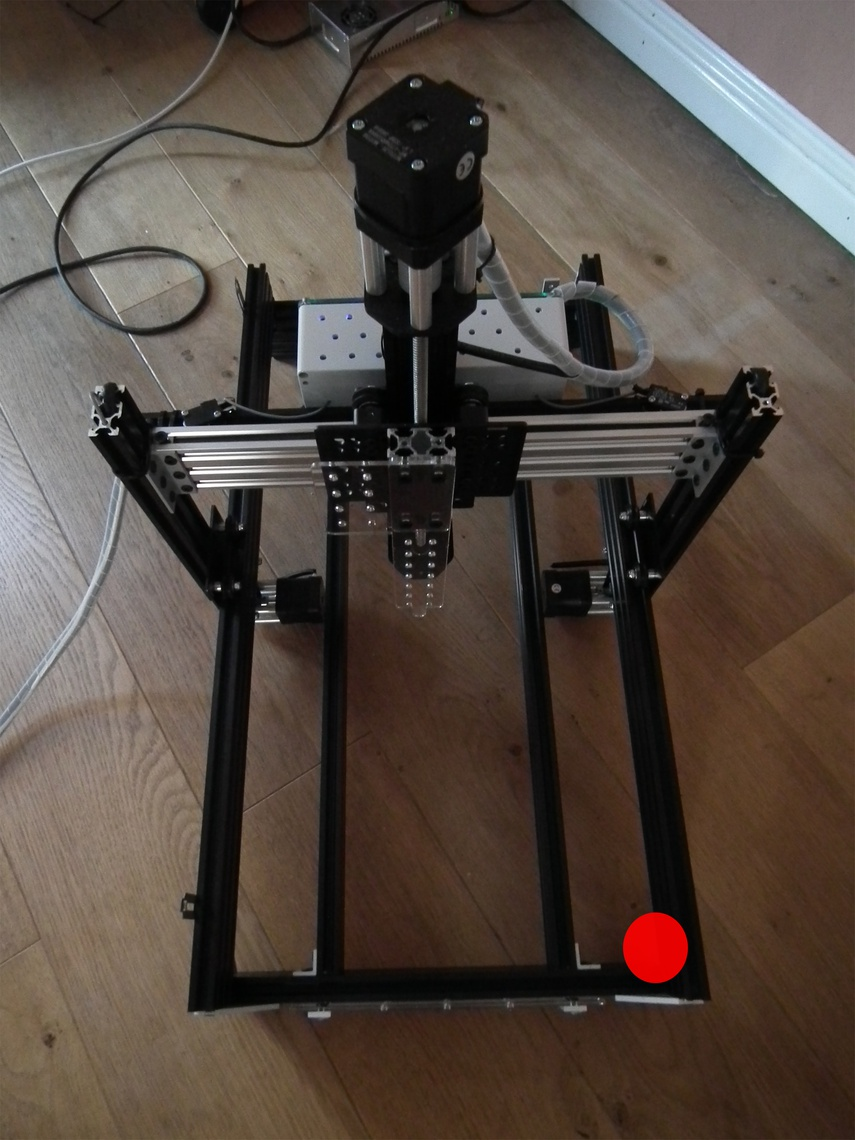
\includegraphics[width=0.75\linewidth]{images/xy_origin} 

}

\caption{Origin of XY coordinate system.}\label{fig:xyOrigin}
\end{figure}

\begin{figure}

{\centering 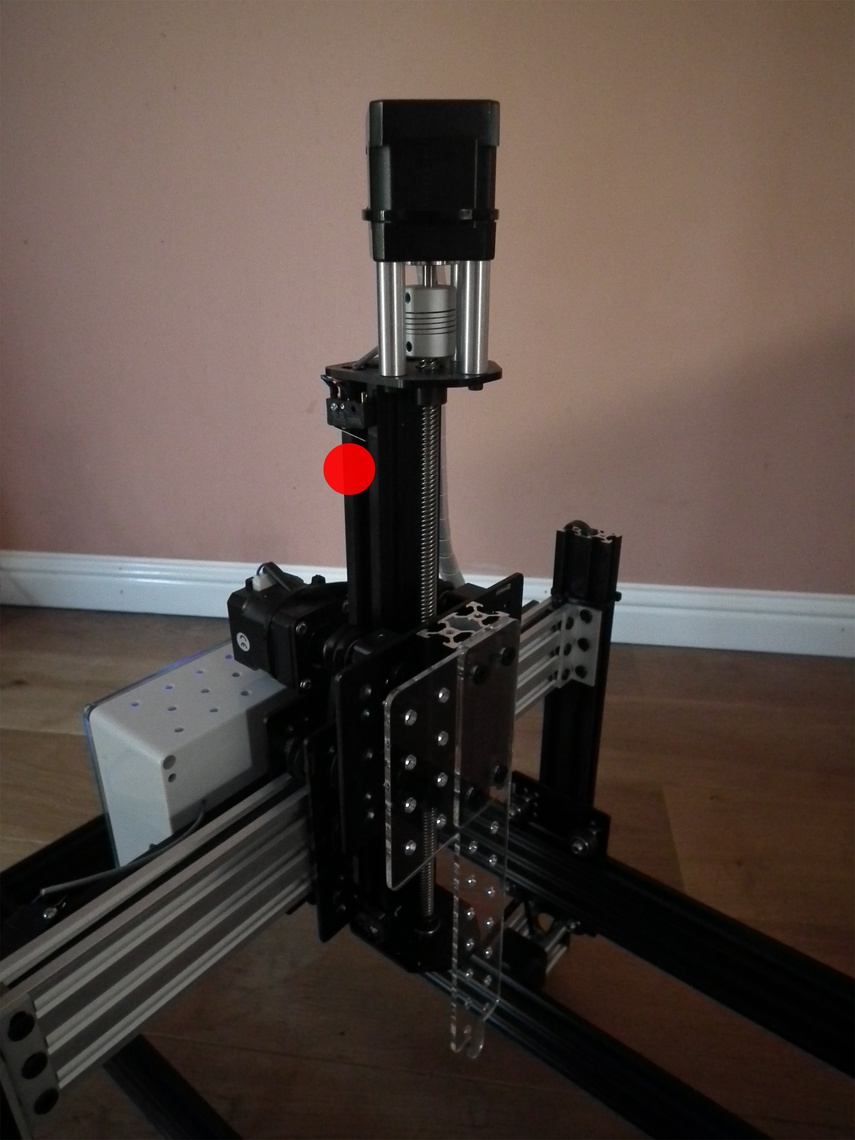
\includegraphics[width=0.75\linewidth]{images/z_origin} 

}

\caption{Origin of Z axis.}\label{fig:zOrigin}
\end{figure}

We also need to set \textbf{\$24}
\href{https://github.com/gnea/grbl/wiki/Grbl-v1.1-Configuration\#24---homing-feed-mmmin}{homing
feed rate} and \textbf{\$25}
\href{https://github.com/gnea/grbl/wiki/Grbl-v1.1-Configuration\#25---homing-seek-mmmin}{homing
seek rate}. Homing seek rate is the initial speed at which Grbl searches
for the limit switches. Once it has them, it makes slower approach at
the homing feed rate to get a more precise location for machine zero. We
will set homing seek rate to 1000 mm/min \texttt{\$24=100} and homing
feed rate to 100 mm/min \texttt{\$25=1000}.

At the end of a homing cycle each actuator carriage must be moved off
its home limit switch, otherwise the hard limit will be triggered. The
\textbf{\$27}
\href{https://github.com/gnea/grbl/wiki/Grbl-v1.1-Configuration\#27---homing-pull-off-mm}{Homing
pull-off (mm)} specifies the distance required to clear the limit
switches. For our robot we will use a value of 5mm:

\begin{verbatim}
$27=5
\end{verbatim}

\emph{\textbf{NOTE: }}

\subsection{Motor step size}\label{motor-step-size}

\textbf{\$100}, \textbf{\$101} and \textbf{\$102} define
\href{https://github.com/gnea/grbl/wiki/Grbl-v1.1-Configuration\#100-101-and-102--xyz-stepsmm}{{[}X,Y,Z{]}
steps/mm}. Suitable values for our stepper motors are:

\begin{verbatim}
$100=40
$101=40
$102=49.673
\end{verbatim}

If you are using a different type of stepper motor, the step size can be
easily calculated by measuring how far each actuator moves in response
to a G-code command. For example, we would calculate the step size for
the X actuator as follows.

\begin{enumerate}
\def\labelenumi{\arabic{enumi}.}
\item
  Using the serial monitor in the Arduino IDE, issue the following
  command to \emph{home} the machine:

\begin{verbatim}
$h
\end{verbatim}
\item
  Read the current position of the machine, as reported by the Grbl
  controller:

\begin{verbatim}
?
\end{verbatim}

  After homing the cartesian coordinates should be zero minus the homing
  pull-off:
\end{enumerate}

\begin{itemize}
\tightlist
\item
  x = -5
\item
  y = -5
\item
  z = -5
\end{itemize}

\begin{enumerate}
\def\labelenumi{\arabic{enumi}.}
\setcounter{enumi}{2}
\item
  Make a note of the physical position of the nozzle.
\item
  Issue a g-code command to move to the -100mm position on the x-axis:

\begin{verbatim}
x-100
\end{verbatim}

  Keep decreasing the value of x until the x-actuator carriage almost
  meets the limit switch on the right hand side of the machine. The
  greater the distance moved, the more precise our calculation of
  step-size will be.
\item
  Query Grbl's machine coordinates:

\begin{verbatim}
?
\end{verbatim}
\item
  Measure the physical distance travelled along the x-axis in
  millimetres.
\item
  Find \textbf{\$100}, the currently configured step size for the
  x-axis:

\begin{verbatim}
$$
\end{verbatim}
\item
  Calculate the correct value for step-size:
\end{enumerate}

\begin{verbatim}
current_step_size = steps/mm in current configuration
grbl_start = start position reported by Grbl controller (mm)
grbl_end = end position reported by Grbl controller (mm)
physical_distance = physical distance moved by actuator (mm)

steps/mm = -(curr_steps_per_mm * (end_pos_grbl-start_pos_grbl)) / physical_distance
\end{verbatim}

\subsection{Feed rates and
acceleration}\label{feed-rates-and-acceleration}

\textbf{\$110}, \textbf{\$111} and \textbf{\$112} set the
\href{https://github.com/gnea/grbl/wiki/Grbl-v1.1-Configuration\#110-111-and-112--xyz-max-rate-mmmin}{maximum
rates (mm/min)} for the X, Y and Z actuators, respectively. We will use
the following values:

\begin{verbatim}
$110=5000
$111=5000
$112=2500
\end{verbatim}

\href{https://github.com/gnea/grbl/wiki/Grbl-v1.1-Configuration\#120-121-122--xyz-acceleration-mmsec2}{Acceleration
(mm/sec\^{}2)} is set to 50 for all axes:

\begin{verbatim}
$120=50
$121=50
$122=50
\end{verbatim}

\subsection{Summary of settings}\label{summary-of-settings}

\begin{verbatim}
$0=10
$1=25
$2=0
$3=5
$4=0
$5=0
$6=0
$10=1
$11=0.010
$12=0.002
$13=0
$20=0
$21=1
$22=1
$23=0
$24=100.000
$25=1000.000
$26=250
$27=5.000
$30=1000
$31=0
$32=0
$100=40.000
$101=40.000
$102=49.673
$110=5000.000
$111=5000.000
$112=2500.000
$120=50.000
$121=50.000
$122=50.000
$130=200.000
$131=500.000
$132=200.000
\end{verbatim}

\section{Setting motor current}\label{setting-motor-current}

The gShield has trimpots for adjusting the motor current of each axis,
as shown in Figure \ref{fig:gShield}.

\begin{figure}

{\centering 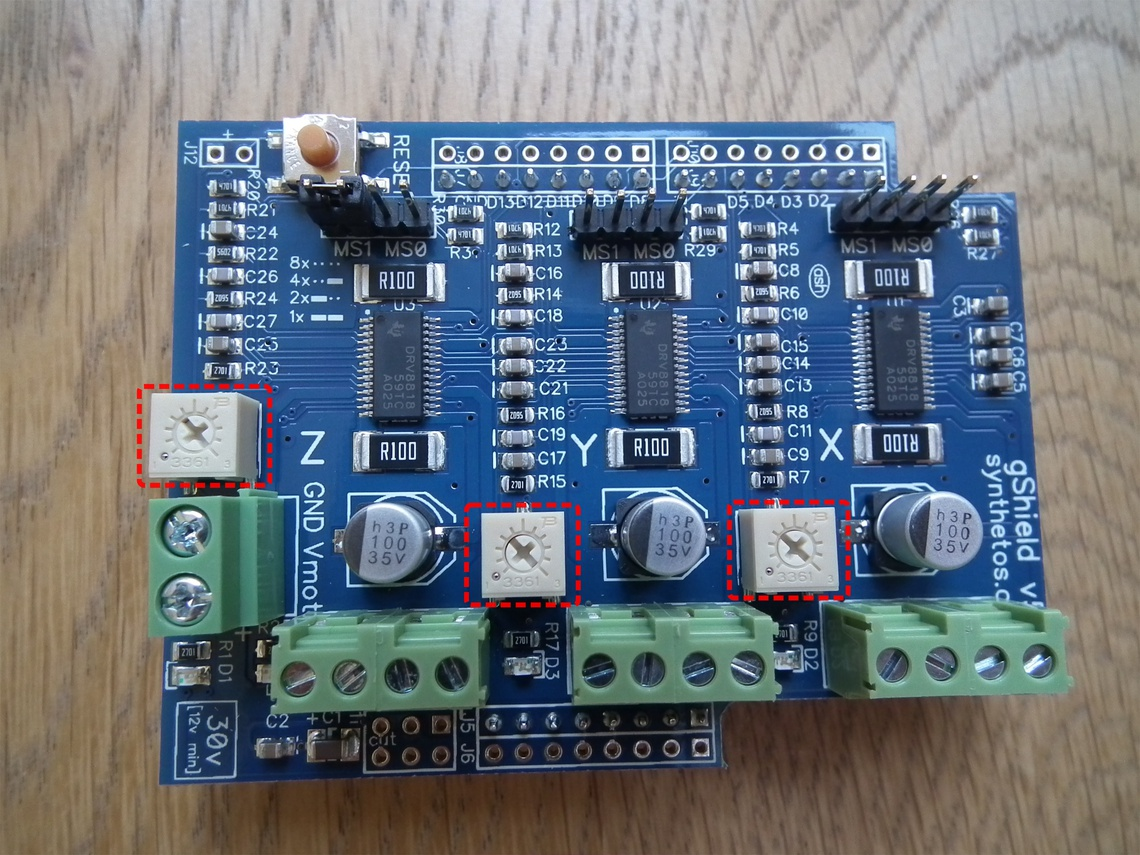
\includegraphics[width=0.75\linewidth]{images/gShield-trimpots} 

}

\caption{gShield trimpots}\label{fig:gShield}
\end{figure}

Instructions for setting motor current are provided here:
\url{https://github.com/synthetos/grblShield/wiki/Using-grblShield\#setting-motor-current}

\chapter{Raspberry Pi setup}\label{raspberry-pi-setup}

\section{Install image}\label{install-image}

The first step is to install Adafruit's custom raspberry pi image on the
micro SD card. The custom image is described here:

\url{https://learn.adafruit.com/adafruit-pitft-28-inch-resistive-touchscreen-display-raspberry-pi/easy-install}

We want the classic version which boots into X by default, rather then
the lite version that boots to the command line. The classic version can
be downloaded from this link:

\url{https://s3.amazonaws.com/adafruit-raspberry-pi/2016-10-18-pitft-28r.zip}

Instructions on installing images on SD cards can be found here:

\url{https://www.raspberrypi.org/documentation/installation/installing-images/}

\section{Network configuration}\label{network-configuration}

The small screen of the pitft makes using most applications quite
tricky. Therefore the first thing we should do after installing the
image is configure networking, so that we can access the raspberry pi
remotely using ssh.

To set a static IP address for the ethernet adapter, add the following
lines to \texttt{/etc/dhcpcd.conf}:

\begin{verbatim}
interface eth0

static ip_address=192.168.1.3/24
static routers=192.168.1.254
static domain_name_servers=192.168.1.254
\end{verbatim}

\textbf{ip\_address}, \textbf{routers} and
\textbf{domain\_name\_servers} should be set to values appropriate for
your network.

To raspberry pi can then be accessed using ssh, \emph{e.g.}:

\begin{verbatim}
  ssh pi@192.168.1.3
\end{verbatim}

The default password for the \textbf{pi} user account is
\textbf{raspberry}

\section{Install minicom}\label{install-minicom}

Minicom is useful for manual control of the robot and for editing grbl
settings. To install minicom run these two commands:

\begin{verbatim}
sudo apt-get update
sudo apt-get install minicom
\end{verbatim}

Before we can use minicom we need to enable serial:

\begin{verbatim}
sudo nano /boot/config.txt
\end{verbatim}

Change the last line of this file from

\begin{verbatim}
enable_uart=0
\end{verbatim}

to

\begin{verbatim}
enable_uart=1
\end{verbatim}

Once serial is enabled we can connect to the grbl controller running on
the arduino by using:

\begin{verbatim}
sudo minicom -D /dev/ttyACM0 -b115200
\end{verbatim}

\section{Expand filesystem}\label{expand-filesystem}

Expand filesystem on micro SD card:

\begin{verbatim}
    sudo raspi-config
    (expand filesystem)
    sudo reboot
\end{verbatim}

\section{Install robot software}\label{install-robot-software}

Make sure you are in pi's home directory:

\begin{verbatim}
cd
\end{verbatim}

Download and unpack robot.tar.gz

\begin{verbatim}
curl -O https://raw.githubusercontent.com/WaylandM/fly-food-robot/master/raspberrypi/robot.tar.gz
tar xzvf robot.tar.gz
\end{verbatim}

The \textbf{robot} directory contains two subdirectories: \textbf{nc}
(g-code scripts) and \textbf{py} (python scripts).

To automatically launch the robot GUI when the raspberry pi starts up,
we need to edit the autostart file for the pi user:

\begin{verbatim}
sudo nano /home/pi/.config/lxsession/LXDE-pi/autostart
\end{verbatim}

Add the following line to autostart:

\begin{verbatim}
@/home/pi/robot/py/fly_gui.py
\end{verbatim}

\chapter{Creating jobs in G-code}\label{creating-jobs-in-g-code}

Running job without GUI - for testing

\chapter{Operation}\label{operation}

\section{Loading boxes of vials}\label{loading-boxes-of-vials}

\bibliography{packages.bib,book.bib}


\end{document}
